\chapter[Fonction de plusieurs variables \life \eng]{Fonctions de plusieurs variables\\ \life \eng}\label{chapFonctPlusVar}

\compileTHEO{

Nous débutons ce chapitre par l'étude du domaine et de l'image des
fonctions de plusieurs variables; en particulier, des fonctions à
valeurs réels définies sur $\RR^2$.  Nous montrons comment utiliser
les {\em sections verticales} et {\em courbes de niveaux} pour
visualiser les fonctions à valeurs réels définies sur $\RR^2$.
Nous abordons par la suite l'étude de la limite d'une fonction de plusieurs
variables en un point ainsi que la continuité des fonctions de
plusieurs variables.  Nous verrons qu'il est beaucoup plus difficile de
déterminer si une fonction de plusieurs variables à une limite en un
point qu'il ne l'est de déterminer si une fonction d'une seule
variable à une limite en un point.

\section{Definitions}

\begin{focus}{\dfn} \index{Fonction!de plusieurs variables}
Une {\bfseries fonction} $f$ de $n$ variables ($n>1$) est une
opération d'un sous-ensemble $D$ de $\RR^n$ à l'ensemble
$\RR^m$ ($m\geq 1$) qui, à chaque élément de $D$, associe un seul
élément de $\RR^m$.  Nous écrivons $f:D\rightarrow \RR^m$ pour désigner une
fonction $f$ de $D\subset \RR^n$ dans $\RR^m$.
\end{focus}

Les fonctions $f:D \rightarrow \RR^m$ où $D\subset \RR^n$ sont
généralement définies par $m$ fonctions $f_i:\RR^n\rightarrow \RR$
pour $i=1$, $2$, \ldots, $m$.  Lorsque nous écrivons
$\VEC{y} = f(\VEC{x})$, nous résumons la formule suivante.
\[
\begin{pmatrix}
y_1 \\ y_2 \\ \vdots \\ y_m
\end{pmatrix}
=
\begin{pmatrix}
f_1(x_1,x_2,\ldots,x_n) \\ f_2(x_1,x_2,\ldots,x_n) \\
\vdots \\ f_m(x_1,x_2,\ldots,x_n)
\end{pmatrix} \; .
\]
Nous écrivons aussi $y_i = f_i(x_1,x_2, \ldots, x_n)$ for $i=1$, $2$,
\ldots, $m$.

Les définitions du domaine et de l'image d'une fonction que nous avons
vu pour les fonctions d'une variable prennent la forme suivante dans
le cas d'une fonction de plusieurs variables.

\begin{focus}{\dfn}
Le {\bfseries domaine}\index{Fonction!domaine} d'une fonction
$f:D \rightarrow \RR^m$ est l'ensemble $D \subset \RR^n$ où la fonction $f$
est définie.  Nous écrivons
\[
\DO f = D \; .
\]
L'{\bfseries image} d'une fonction $f:D \rightarrow \RR^m$ est
l'ensemble des éléments $\VEC{y} \in \RR^m$ pour lesquels il existe au
moins un élément $\VEC{x} \in D$ tel que $f(\VEC{x}) = \VEC{y}$.
\index{Fonction!image}  Nous écrivons
\begin{align*}
\IM f &\equiv \left\{ \VEC{y} \in \RR^m : f(\VEC{x}) = \VEC{y}
\text{ pour au moins un élément } \VEC{x} \in D \right\} \; .
\end{align*}
\end{focus}

\begin{rmkList}
\begin{enumerate}
\item Pour être consistant avec la notation algébrique, nous devrions
représenter l'argument $\VEC{x} \in \RR^n$ d'une fonction par la matrice
\[
\VEC{x} = \begin{pmatrix} x_1 \\ x_2 \\ \vdots \\ x_n
\end{pmatrix}
\]
de dimension \nm{n}{1}.  Par contre, la tradition veut que nous
utilisons la notation géométrique
\[
\VEC{x} = \left(x_1 , x_2 , \ldots , x_n \right)
\]
pour les fonctions à valeurs réelles sur $\RR^n$.  Le lecteur devrait
toujours garder en tête la notation algébrique car c'est celle-ci qui
doit être utilisée pour l'étude des fonctions de $\RR^n$ dans $\RR^m$
où $m>1$.
\item Nous avons
\[
\DO f = \bigcap_{i=1}^m \DO f_i \; .
\]
C'est-à-dire que $f$ est définie au point $\VEC{x}$ si tous les
$f_i$'s sont définis au point $\VEC{x}$.
\end{enumerate}
\end{rmkList}

Sans en être conscient, nous avons déjà travaillé avec des fonctions
de $\RR^n$ dans $\RR^m$.  Commençons donc par revoir ces fonctions.

Soit $A$ une matrice de dimension \nm{m}{n}.  Nous pouvons utiliser cette
matrice pour définir une fonction $f:\RR^n\rightarrow \RR^m$ de la
façon suivante.
\[
f(\VEC{x}) = A\VEC{x}
\]
pour tout $\VEC{x} \in \RR^n$.  Ainsi, cette fonction associe à un
vecteur $\VEC{x}$ dans $\RR^n$ le vecteur $\VEC{y} = A\VEC{x}$ dans
$\RR^m$.  Les fonctions $f:\RR^n\rightarrow \RR^m$ définies par le
produit d'une matrice avec un vecteur satisfont la définition
suivante.

\begin{focus}{\dfn}
Une fonction $f:\RR^n\rightarrow \RR^m$ est appelée une
{\bfseries fonction linéaire}\index{Fonction linéaire} ou
{\bfseries application linéaire}\index{Application linéaire} si
elle satisfait les deux propriétés suivantes:
\begin{enumerate}
\item $f(\alpha\,\VEC{x}) = \alpha f(\VEC{x})$ pour tout vecteur
$\VEC{x} \in \RR^n$ et tout $\alpha \in \RR$.
\item $f(\VEC{x}+\VEC{y}) = f(\VEC{x}) + f(\VEC{y})$ pour tous vecteurs
$\VEC{x}$ et $\VEC{y}$ de $\RR^n$. 
\end{enumerate}
\label{funct_lin_def} 
\end{focus}

\begin{egg}
La matrice
\[
R_\theta =
\begin{pmatrix}
\cos(\theta) & -\sin(\theta) \\ \sin(\theta) & \cos(\theta)
\end{pmatrix}
\]
défini une fonction linéaire $f:\RR^2\rightarrow \RR^2$ par
$f(\VEC{x})=R_\theta \VEC{x}$ pour tout $\VEC{x}\in \RR^2$.

Essayons de voir quelle est l'action de cette fonction sur un vecteur
$\displaystyle \VEC{x} = \begin{pmatrix} x_1 \\ x_2 \end{pmatrix}$.
Nous avons
\[
\VEC{y} = f(\VEC{x}) = R_\theta \VEC{x} =
\begin{pmatrix}
\cos(\theta) & -\sin(\theta) \\ \sin(\theta) & \cos(\theta)
\end{pmatrix}
\begin{pmatrix} x_1 \\ x_2 \end{pmatrix}
= \begin{pmatrix}
x_1\,\cos(\theta) -x_2\,\sin(\theta) \\ x_1\,\sin(\theta) +x_2\, \cos(\theta)
\end{pmatrix} \; .
\]
Le vecteur $\VEC{y}$ est de même longueur que $\VEC{x}$. car
\begin{align*}
\|\VEC{y}\| &= \sqrt{\big(x_1\,\cos(\theta) -x_2\,\sin(\theta)\big)^2 
+\big(x_1\,\sin(\theta) +x_2\, \cos(\theta)\big)^2} \\
&=\sqrt{ x_1^2\big(\cos^2(\theta)+\sin^2(\theta)\big) +
x_2^2\big(\cos^2(\theta)+\sin^2(\theta)\big)}
= \sqrt{ x_1^2 + x_2^2 } = \|\VEC{x}\|
\end{align*}
où nous avons évidemment utilisé l'identité trigonométrique
$\cos^2(\theta) + \sin^2(\theta) =1$ pour tout $\theta$.  De plus,
\begin{align*}
\ps{\VEC{x}}{\VEC{y}}
&= \VEC{x}^\top \VEC{y}
= \begin{pmatrix} x_1 & x_2 \end{pmatrix}
\begin{pmatrix}
x_1\,\cos(\theta) -x_2\,\sin(\theta) \\ x_1\,\sin(\theta) +x_2\, \cos(\theta)
\end{pmatrix} \\
&= (x_1^2+x_2^2)\cos(\theta)
= \|\VEC{x}\|\,\|\VEC{y}\| \cos(\theta) \; .
\end{align*}
C'est exactement la formule (\ref{CosVectors}) qui détermine le
cosinus de l'angle entre les vecteurs $\VEC{x}$ et $\VEC{y}$.  L'angle
entre les vecteurs $\VEC{x}$ et $\VEC{y}$ est donc $\theta$.

L'image par $f$ d'un vecteur $\VEC{x}$ est donc la rotation par
$\theta$ radians du vecteur $\VEC{x}$ (figure~\ref{ROTA}).  Nous avons
une rotation dans le sens contraire aux aiguilles d'une montre quand
$\theta>0$ et une rotation dans le sens des aiguilles d'une montre
quand $\theta<0$.

Par exemple, si
$\displaystyle \VEC{x} = \begin{pmatrix} \sqrt{3} \\ 1 \end{pmatrix}$
et $\theta=\pi/3$, alors
\[
\VEC{y}= f(\VEC{x}) = R_{\pi/3}\VEC{x}
= \begin{pmatrix} 1/2 & -\sqrt{3}/2 \\ \sqrt{3}/2 & 1/2 \end{pmatrix}
\begin{pmatrix} \sqrt{3} \\ 1 \end{pmatrix}
= \begin{pmatrix} 0 \\ 2 \end{pmatrix} \; .
\]
$\VEC{x}$ et $\VEC{y}$ sont deux vecteurs de longueur $2$.  Le vecteur
$\VEC{y}$ est le résultat d'une rotation dans le sens contraire aux
aiguilles d'une montre par $\pi/3$ radians de $\VEC{x}$; le vecteur
$\VEC{x}$ forme un angle de $\pi/6$ avec l'axe des $x$ alors que
$\VEC{y}$ forme un angle de $\pi/2$ avec l'axe des $x$.
\end{egg}

\PDFfig{14_var_mult_fonct/rot}{Rotation d'un vecteur dans le plan}{Le
vecteur $\VEC{y}$ est obtenu par une rotation de $\theta$ radians dans
le sens contraire aux aiguilles d'une montre du $\VEC{x}$.}{ROTA}

\begin{egg}
Nous avons déjà travaillé avec des fonctions de la forme
$f:\RR^n\rightarrow \RR^m$.  Les représentations paramétriques des
courbes dans $\RR^m$ sont des fonctions de $\RR$ dans $\RR^m$.  C'est
le cas où $n=1$.

Par exemple, la fonction $\phi:\RR\rightarrow \RR^3$ définie par les
fonctions
\[
\phi_1(t) = 2\,\cos(t) \quad , \quad
\phi_2(t) = 2\,\sin(t) \quad \text{et} \quad
\phi_3(t) = t
\]
pour $t \in \RR$ est une représentation paramétrique d'un ressort
de longueur infinie (car $\phi$ est définie pour tout $t\in \RR$) dont
l'axe central est l'axe des $x_3$.
\end{egg}

\begin{egg}
Les fonctions
\[
f_1(x_1,x_2,x_3) = x_1\,x_2 \sin(x_1^2+x_2^2+x_3^2)
\quad \text{et} \quad
f_2(x_1,x_2,x_3) = \frac{x_1\,x_2\,x_3}{x_1^2+x_2^2+x_3^2}
\]
définissent une fonction $f:D\rightarrow \RR^2$ où
$D = \{\VEC{x} \in \RR^3 : \VEC{x} \neq \VEC{0}\}$.  Le vecteur
$\VEC{y} = f(\VEC{x})$ possède les coordonnées
\[
y_1 = f_1(x_1,x_2,x_3)= x_1\,x_2 \sin(x_1^2+x_2^2+x_3^2)
\quad \text{et} \quad
y_2 = f_2(x_1,x_2,x_3)= \frac{x_1\,x_2\,x_3}{x_1^2+x_2^2+x_3^2} \; .
\]
le domaine $D \subset \RR^3$ de la fonction $f:D\rightarrow \RR^2$ est
\[
D = \{ \VEC{x} \in \RR^3 : \VEC{x} \neq \VEC{0} \}
\]
car $f_2$ n'est pas définie pour $\VEC{x} = \VEC{0}$.
\end{egg}

\section{Fonctions de plusieurs variables à valeurs réelles}

Dans cette section, nous considérons les fonctions à valeurs réelles;
c'est-à-dire, $m=1$.

\begin{egg}
La température maximale (en degrés centigrades) au point de longitude
$x_1$ et latitude $x_2$ (en degrés) définit une fonction $T:D \rightarrow \RR$
qui à chaque point de coordonnées $(x_1,x_2)$ associe la température
maximale $T(x_1,x_2)$ à ce point.  L'ensemble $D$ est l'ensemble des
coordonnées; c'est-à-dire,
\[
D = \{ (x_1,x_2) : 0\leq x_1 \leq 360 \quad \text{et} \quad
-90 \leq x_2 \leq 90 \}
\]
où nous supposons que $x_2<0$ dans l'hémisphère sud.
\end{egg}

\begin{egg}
Une fonction de plusieurs variables peut être définie à l'aide d'un
tableau comme c'est le cas dans le tableau suivant qui donne l'indice
de température en fonction de la température et du niveau d'humidité.
\[
\begin{array}{lc|ccc}
& & \multicolumn{3}{c}{\text{Température en C}^\circ}\\
& & 20 & 22 & 24 \\
\hline
& 0 & 18 & 20 & 22 \\
& 10 & 19 & 21 & 23 \\
& 20 & 19.5 & 21.5 & 23.5 \\
& 30 & 20 & 22 & 25 \\
& & & & \\
\begin{rotate}{90}\text{Humidité en \%}\end{rotate} & & & &
\end{array}
\]
Ce tableau définit une fonction $I:D \rightarrow \RR$ où
\[
D = \{ (x_1,x_2) : x_1=20, 22, 24 \quad \text{et} \quad
x_2= 0, 10, 20, 30 \} \; .
\]
Nous avons $I(0,22) = 20^\circ$C, $I(20,22) = 21.5^\circ$C, etc.
\end{egg}

\begin{egg}
Nous pouvons définir une fonction à l'aide d'une expression algébrique.
Par exemple,
\[
f(x_1,x_2) = \sqrt{36-4x_1^2-9x_2^2}
\]
définit une fonction sur l'ensemble des points $(x_1,x_2)$ tels que
$36-4x_1^2-9x_2^2 \geq 0$.  Ainsi, $f:D\rightarrow \RR$ où 
\[
D = \{ (x_1,x_2) : 4x_1^2+9x_2^2 \leq 36 \} \; .
\]
C'est la région du plan bornée par l'ellipse
$\displaystyle \frac{x_1^2}{3^2} + \frac{x_2^2}{2^2} = 1$.
\label{egg_ellipsoid}
\end{egg}

Pour les fonctions de plusieurs variables, la définition du graphe
d'une fonction s'énonce de la façon suivante.

\begin{focus}{\dfn} \index{Fonction!graphe}
Soit $f:D\rightarrow \RR$ une fonction définit sur un sous-ensemble
$D\subset \RR^n$.  Nous définissons le {\bfseries graphe de la fonction}
$f$ comme étant l'ensemble
\[
\text{graphe de }f = \left\{ (x_1,x_2,\ldots,x_n, f(x_1,x_2,\ldots,x_n))
: (x_1,x_2,\ldots,x_n) \in D \right\}
\]
de $\RR^{n+1}$.
\end{focus}

Seules les fonctions définies sur un ensemble $D \subset \RR^2$
pourront être représentées par un dessin (certainement dans l'univers
de l'auteur).  Nous retrouvons à la figure~\ref{D3_GRAPH} le
graphe d'une possible fonction
$f:D \rightarrow \RR$ où $D\subset \RR^2$.  

\PDFfig{14_var_mult_fonct/d3_graph}{Le graphe d'une fonction de
$D \subset \RR^2$ dans $\RR$}{Pour obtenir le graphe $S$ de la fonction
$f$, nous traçons dans le système de coordonnées cartésiennes l'ensemble
des points $(x_1,x_2,f(x_1,x_2))$ pour $(x_1,x_2) \in D$.}{D3_GRAPH}

\begin{focus}{\dfn} \index{Fonction affine}
Les {\bfseries fonctions affines} sont les fonctions
$f:\RR^n \to \RR^m$ de la forme $f(\VEC{x}) = A \VEC{x} + \VEC{b}$
pour $A$, une matrice de dimension \nm{n}{m}, et $\VEC{b} \in \RR^m$,
un vecteur arbitraire mais fixe.  Si $\VEC{b}=0$, nous obtenons une
fonction linéaire de $\RR^n$ dans $\RR^m$ puisque $f$ satsifait alors
la définition~\ref{funct_lin_def}.

En particulier, si $f:\RR^n \to \RR$, la fonction $f$ est de la forme
$\displaystyle f(x,y) = \sum_{i=1}^n m_i\,x_i +b$ où les $m_i$ et
$b$ sont des constantes.
\end{focus}

Dans le cas d'une fonction affine $f:\RR^2 \to \RR$, nous observons que le
graphe de $f$ est un plan dans l'espace.

\begin{egg}
Le tableau suivant donne quelques valeurs d'une fonction affine $f$.
Cherchons une formule pour cette fonction.
\[
\begin{array}{c|c|c|c|c}
x_2 \backslash \raisebox{1ex}{$x_1$} & 0 & 1 & 2 & 3 \\
\hline
-1 & 1.5 & 3.5 & 5.5 & 7.5 \\
\hline
0 & 1 & 3 & 5 & 7 \\
\hline
1 & 0.5 & 2.5 & 4.5 & 6.5 \\
\hline
2 & 0 & 2 & 4 & 6
\end{array}
\]

Comme le graphe de $f$ est un plan, il suffit de chercher une formule
de la forme suivante pour $f$.
\begin{equation}\label{eggEquPlan}
  x_3 = f(x_1,x_2)=m_1 x_1 + m_2 x_2 + b \ .
\end{equation}
Nous présentons deux méthodes pour déterminer les valeurs de $m_1$,
$m_2$ et $b$.  La première méthode est géométrique alors que la
deuxième est purement algébrique.

\begin{enumerate}
\item  Comme l'intersection de deux plans non parallèles est une droite,
l'intersection du graphe de $f$ et du plan $x_1=1$ est une droite qui
contient les points $(x_2,x_3) = (-1, 3.5)$, $(0,3)$, $(1,2.5)$ et
$(2,2)$.  C'est donc une droite de pente
$(3.5-3)/(-1-0) = -0.5$.  Or, si on pose $x_1=1$ dans
(\ref{eggEquPlan}), nous obtenons la formule
$x_3= m_2 x_2 + m_1 + b$ pour la droite d'intersection.  Donc
$m_2 = -0.5$.

L'intersection du graphe de $f$ et du plan $x_2=2$ est une droite qui
contient les points $(x_1,x_3) = (0, 0)$, $(1,2)$, $(2,4)$ et $(3,6)$.
C'est donc une droite de pente $(2-0)/(1-0) = 2$.
Or, si on pose $x_2=2$ dans (\ref{eggEquPlan}), nous
obtenons la formule $x_3= m_1x_1 + 2 \, m_2 + b$ pour la droite
d'intersection.  Donc $m_1 = 2$.

Il découle des deux paragraphes précédents que
$x_3=f(x_1,x_2) = 2x_1 -0.5 x_2 + b$.  Pour
déterminer $b$, prenons le point $(1,1, 2.5)$ du graphe de $f$ (tout
autre point du graphe serait acceptable).  Donc
$2.5 = f(1,1) = 2 -0.5 + b$.  Ce qui donne $b=1$.

La formule algébrique pour $f$ est $x_3=f(x_1,x_2) = 2x_1-0.5x_2 +1$.
\item Nous savons qu'un plan est déterminé par trois points qui ne
sont pas sur une même droite.  Choisissons les trois
points $(1,-1,3.5)$, $(1,2,2)$ et $(2,1,4.5)$ (tout
autre choix de trois points qui ne sont pas sur une même droite
aurait été aussi valide).
Si nous substituons ces trois points dans la formule
(\ref{eggEquPlan}), nous obtenons les trois équations linéaires
suivantes.
\[
3.5 = m_1- m_2 + b \ , \ 2 = m_1 + 2m_2 + b \quad \text{et} \quad
4.5 = 2 m_1 + m_2 + b \; .
\]
Il faut résoudre ce système d'équations linéaires pour $m_1$,
$m_2$ et $b$.  Sous la forme matricielle, nous avons
\[
\begin{pmatrix} 1 & -1 & 1 \\ 1 & 2 & 1 \\ 2 & 1 & 1 \end{pmatrix}
\begin{pmatrix} m_1 \\ m_2 \\ b \end{pmatrix}
= \begin{pmatrix} 3.5 \\ 2 \\ 4.5 \end{pmatrix} \; .
\]
La matrice augmentée est
\[
\left(\begin{array}{rrr|r}
1 & -1 & 1 & 3.5 \\
1 & 2 & 1 & 2 \\
2 & 1 & 1 & 4.5
\end{array}\right) \; .
\]
$R_2-R_1 \to R_2$ et $R_3 -2R_1 \to R_3$ donnent
\[
\left(\begin{array}{rrr|r}
1 & -1 & 1 & 3.5 \\
0 & 3 & 0 & -1.5 \\
0 & 3 & -1 & -2.5
\end{array}\right) \; .
\]
$R_3-R_2 \to R_3$ donne
\[
\left(\begin{array}{rrr|r}
1 & -1 & 1 & 3.5 \\
0 & 3 & 0 & -1.5 \\
0 & 0 & -1 & -1
\end{array}\right) \; .
\]
$(1/3)R_2 \to R_2$ et $-R_3\to R_3$ donnent
\[
\left(\begin{array}{rrr|r}
1 & -1 & 1 & 3.5 \\
0 & 1 & 0 & -0.5 \\
0 & 0 & 1 & 1
\end{array}\right) \; .
\]
$R_1+R_2 -R_3 \to R_1$ donne
\[
\left(\begin{array}{rrr|r}
1 & 0 & 0 & 2 \\
0 & 1 & 0 & -0.5 \\
0 & 0 & 1 & 1
\end{array}\right) \; .
\]
Nous trouvons donc $m_1=2$, $m_2 = -1/2$ et $b=1$ comme pour la première
méthode.
\end{enumerate}
\end{egg}

\begin{egg}
À l'exemple~\ref{egg_ellipsoid}, le domaine de $f$ est
\[
\DO f = \{ (x_1,x_2) : \frac{x_1^2}{3^2} + \frac{x_2^2}{2^2} \leq 1 \} \; .
\]
Montrons que l'image de $f$ est l'intervalle $[0,6]$.

Si nous posons $x_3 = \sqrt{36-4x_1^2-9x_2^2}$, nous obtenons l'équation de
l'ellipsoïde $x_3^2 + 4x_1^2 + 9x_2^2 = 36$ qui est dessiné ci-dessous.
\PDFgraph{14_var_mult_fonct/ellipsoid}

La partie de l'ellipsoïde au-dessus du plan $x_3=0$ est le graphe de
$f$.  La plus grande valeur de $f$ est $6$ lorsque $(x_1,x_2)=(0,0)$ et la
plus petite valeur de $f$ est $0$ lorsque $x_1^2/3^2 + x_2^2/2^2 = 1$.  La
fonction $f$ prend toutes les valeurs entre $0$ et $6$.
\end{egg}

\begin{egg}
Traçons le graphe de la fonction
$x_3 = f(x_1,x_2) = 5 - \sqrt{36 - 9(x_1-1)^2 - 4(x_2-2)^2}$.

Après quelques manipulations algébriques, nous obtenons
$(x_3 - 5)^2 + 9(x_1-1)^2 + 4(x_2-2)^2 = 36$.  C'est le même
ellipsoïde qu'à l'exemple précédent sauf qu'il est maintenant centrée
au point $(x_1,x_2,x_3) = (1,2,5)$ et non plus à l'origine.
\PDFgraph{14_var_mult_fonct/ellipsoid2}

Puisque nous avons un signe négatif devant la racine carrée, le graphe de
$f$ est la partie sous le plan $x_3 = 5$.   L'image de $f$ est donc
l'intervalle $[-1,5]$.
\end{egg}

Même pour les fonctions de deux variables, il est souvent fort
difficile de tracer le graphe d'une fonction.  Nous avons donc besoin de
méthodes pour représenter l'information fournie par une fonction.

\begin{focus}{\dfn} \index{Courbe de niveaux}
Soit $f:D\rightarrow \RR$ une fonction définie sur un ensemble
$D\subset \RR^2$.  Une {\bfseries courbe de niveaux} de $f$ est une
courbe $C \subset D$ définie par l'équation $f(x_1,x_2) = k$ où $k$
est une constante; c'est-à-dire,
$\displaystyle C = \{ (x_1,x_2) \in D : f(x_1,x_2) = k \}$.
\end{focus}

En traçant plusieurs courbes de niveau d'une fonction $f$ sur une
même figure, nous pouvons déterminer (approximativement) les maximums
et minimums locaux de cette fonction ainsi que sur les régions où elle
est croissante et décroissante.

\begin{egg}
Traçons plusieurs courbes de niveau pour la fonction
\[
f(x_1,x_2) = \sqrt{36-4x_1^2-9x_2^2} \; .
\]

Si $f(x_1,x_2)=k$, nous obtenons
\[
\frac{x_1^2}{3^2} + \frac{x_2^2}{2^2} = 1- \frac{k^2}{6^2} \; .
\]
Les seules courbes de niveau sont pour $|k| \leq 6$ car
$x_1^2/3^2 + x_2^2/2^2 \geq 0$ pour tout $x_1$ et $x_2$.  Les courbes de
niveau sont des ellipses.  Nous obtenons la figure suivante.
\MATHgraph{14_var_mult_fonct/lev_curves1}{8cm}
\end{egg}

\begin{egg}
Traçons plusieurs courbes de niveau pour la fonction
$f(x_1,x_2) = x_1^2-x_2^2$.

Les courbes de niveau $f(x_1,x_2)=k$ sont
définies pour tout $k$.  Ce sont des hyperboles sauf pour
$k=0$ où nous obtenons les droites $x_2= \pm x_1$.  Nous obtenons la figure
suivante.
\MATHgraph{14_var_mult_fonct/lev_curves2}{8cm}
\end{egg}

% \begin{egg}
% Trouvons le domaine et traçons quelques courbes de niveau pour chacune
% des fonctions suivantes.\\
% \subQ{a} $f(x,y) = \ln(xy-1)$\\
% \subQ{b} $f(x,y) = \sqrt{(x+y)/(x-y)}$
% \end{egg}

\begin{focus}{\dfn}
Soit $f:D\rightarrow \RR^2$ une fonction définie sur un ensemble
$D\subset \RR^2$ et soit $M \subset \RR^3$ un plan défini par
$x_2=m\,x_1+b$.  Une
{\bfseries section verticale}\index{Section Verticale} de $f$ est la
courbe $C \subset M$ définie par l'intersection de $M$ avec le graphe
de $f$; c'est-à-dire,
\[
C = \left\{ \left(x_1, x_2, f(x_1, x_2)\right) : x_2 = m\,x_1+b \text{ et }
(x_1,x_2) \in D \right\} \; .
\]
\end{focus}

Deux familles de plans verticaux sont généralement utilisées pour
produire des sections verticales: les plans $x_1=k_1$ et $x_2=k_2$ où
$k_1$ et $k_2$ sont des constantes.

\begin{egg}
Décrivons les sections verticales $x_1=k_1$ et $x_2=k_2$ de
$f(x_1,x_2) = x_1^2-x_2^2$.

Si $x_1=k_1$, nous obtenons l'équation $x_3=f(k_1,x_2)=k_1^2-x_2^2$
qui représente des paraboles ouvertes vers le bas.  Si $x_2=k_2$, nous
obtenons l'équation $x_3=f(x_1,k_2)=x_1^2-k_2^2$ qui représente des
paraboles ouvertes vers le haut.  Le graphe de $f$ est donné
ci-dessous.
\MATHgraph{14_var_mult_fonct/vert_sect1}{8cm}
\end{egg}

Nous avons reproduit à la figure~\ref{PLANAR1} quelques courbes
planaires que nous retrouvons fréquemment comme courbes de niveau ou
sections verticales de fonctions.

\PDFfig{14_var_mult_fonct/planar1}{Quelques courbes planaires
élémentaires }{Voici quelques courbes planaires élémentaires qui peuvent
représenter des courbes de niveau ou des sections verticales d'une
fonction.}{PLANAR1}

%\clearpage

\section{Limites et fonctions continues}

La définition de la limite d'un fonction $f:\RR^n \to \RR$ en une
point avec $n>1$ est fondamentalement la même que la définition de la
limite d'une fonction $f:\RR \to \RR$ en un point que nous avons
donnée à la section~\ref{oneD_LimCont}.   De même, La définition de la
continuité d'un fonction $f:\RR^n \to \RR$ en une point avec $n>1$ est
fondamentalement la même que la définition de la continuité d'une
fonction $f:\RR \to \RR$ en une point que nous avons donnée à la
section~\ref{oneD_LimCont}.   La seule différence dans les deux cas
est que la valeur absolue est remplacée par la {\em norme euclidienne}. 

Sur la droite réelle, la distance entre un point $x$ et l'origine est
donnée par la valeur absolue $|x|$ de ce nombre.  La distance entre
deux points $x$ et $y$ est donnée par la valeur absolue $|x-y|$.

La distance euclidienne dans $\RR^n$ joue le rôle de la valeur absolue
dans $\RR$.  Nous avons vu à la définition~\ref{norm} que la longueur d'un
vecteur $\VEC{x} \in \RR^n$ (ou sa
{\bfseries norme euclidienne}\index{Norme euclidienne}) est donnée par 
\[
\| \VEC{x} \| = \sqrt{x_1^2 + x_2^2 + \ldots + x_n^2} \; .
\]
Le symbole $\| \cdot \|$ dans $\RR^n$ remplace le symbole $|\cdot|$
pour la valeur absolue dans $\RR$.
La distance euclidienne entre deux points $\VEC{a}$ et $\VEC{b}$ de
$\RR^n$ est
\[
\|\VEC{a} - \VEC{b} \| = \sqrt{(b_1-a_1)^2 + (b_2-a_2)^2 + \ldots
+ (b_n-a_n)^2} \; .
\]
Une illustration de la distance entre deux points de $\RR^2$ et une
illustration de la longueur d'une vecteur dans $\RR^3$ sont données à la
figure~\ref{EUCLID}.  La formule pour calculer $\| \VEC{a} - \VEC{b} \|$
est bien la distance entre deux points $\VEC{a}$ et $\VEC{b}$
obtenue à l'aide du théorème de Pythagore.

\PDFfig{14_var_mult_fonct/euclid}{La norme Euclidienne dans $\RR^n$}
{Illustrations de la distance entre deux points de $\RR^2$ dans la
dessin à gauche et de la longueur d'un vecteur de $\RR^3$ dans le
dessin à droite.}{EUCLID}

Nous commençons par définir la notion de convergence d'une suite de points
dans $\RR^n$.

\begin{focus}{\dfn}
Nous disons qu'une suite de points
$\displaystyle \left\{\VEC{x}_k\right\}_{k=1}^\infty$ de $\RR^n$
{\bfseries converge (ou tend) vers un point
$\mathbf{\VEC{c} \in \RR^n}$}\index{Suite!convergence dans $\RR^n$} si la
distance euclidienne entre $\VEC{x}_k$ et $\VEC{c}$ approche $0$
lorsque $k$ tend vers plus l'infini.  En d'autres mots,
\[
\lim_{k\rightarrow \infty} \|\VEC{x}_k-\VEC{c}\| = 0 \; .
\]
Nous écrivons
\[
\lim_{k\rightarrow \infty} \VEC{x}_k = \VEC{c} \; .
\]
Nous disons que $\VEC{c}$ est la {\bfseries limite}\index{Suite!limite} de
la suite $\displaystyle \left\{\VEC{x}_k\right\}_{k=1}^\infty$.
\end{focus}

La définition précédente de limite d'une suite est équivalente à la
définition suivante en termes de $\epsilon$ et $\delta$.

\begin{focus}[\theory]{\dfn}
Nous disons qu'une suite de points 
$\displaystyle \left\{\VEC{x}_k\right\}_{k=1}^\infty$ de $\RR^n$
{\bfseries converge (ou tend) vers un point
$\mathbf{\VEC{c} \in \RR^n}$}\index{Suite!convergence} si,
{\em quel que soit $\epsilon >0$}, il existe un entier $K>0$ (qui peut
dépendre de $\epsilon$) tel que
\[
\| \VEC{x}_k - \VEC{c} \| < \epsilon \qquad \text{si} \qquad k>K \; .
\]
Nous écrivons
\[
\lim_{k\rightarrow \infty} \VEC{x}_k = \VEC{c} \; .
\]
Nous disons aussi que $\VEC{c}$ est la {\bfseries limite}\index{Suite!limite}
de la suite $\displaystyle \left\{\VEC{x}_k\right\}_{k=1}^\infty$.
\end{focus}

Avant de définir la limite, la continuité et la dérivée d'une fonction
de plusieurs variables à un point, il faut généraliser le concept
d'intervalles que nous retrouvons sur la droite réelle.

\begin{focus}{\dfn}
Un sous-ensemble $V \subset \RR^n$ est
{\bfseries ouvert}\index{Ensemble ouvert} si,
{\em quel que soit $\VEC{v} \in V$}, nous pouvons trouver $\delta>0$ (qui
peut dépendre de $\VEC{v}$) tel que
\[
B_\delta(\VEC{v}) = \{ \VEC{x} \in \RR^n : \|\VEC{x} - \VEC{v}\| <
\delta \} \subset V \; .
\]
$\displaystyle B_\delta(\VEC{v})$ est la boule de rayon $\delta$
centrée au point $\VEC{v}$ (figure~\ref{VOISIN}).

Un sous-ensemble $V \subset \RR^n$ est un
{\bfseries voisinage}\index{Voisinage} d'un
point $\VEC{c} \in \RR^n$ si $\VEC{c} \in V$ et $V$ est ouvert.
L'ensemble $V\setminus \{\VEC{c}\}$, l'ensemble $V$ auquel nous avons enlevé
le point $\VEC{c}$, est alors appelé un
{\bfseries voisinage troué}\index{Voisinage troué} de $\VEC{c}$.
\end{focus}

Notons que les boules $B_\delta(\VEC{v})$ ne contiennent pas leur
frontière $\{ \VEC{x} \in \RR^n : \|\VEC{x}-\VEC{c} \| = \delta \}$.
Ainsi, si $V$ est un sous-ensemble ouvert de $\RR^n$, nous pouvons conclure
qu'une fonction $f:V\rightarrow \RR$ est définie \flqq autour\frqq\ de
tout point $\VEC{v} \in V$ (figure~\ref{VOISIN}).  C'est un
détail subtile qui nous permet de bien définir la dérivée
d'une fonction en un point.

\PDFfig{14_var_mult_fonct/voisin}{Voisinage d'un point de $\RR^n$}{$V$
est un voisinage possible pour le point $\VEC{c} \in \RR^2$.  Quel que
soit le point $\VEC{v}$ de $V$ que nous choisissons, nous pouvons toujours
trouver une boule $B_\delta(\VEC{v})$ de rayon $\delta$ centrée à
$\VEC{v}$ qui soit à l'intérieur de $V$.  Plus $\VEC{v}$ sera près de
la frontière de $V$, plus $\delta$ devra être petit.}{VOISIN}

Il est parfois utile de déterminer la frontière d'un sous-ensemble de
$\RR^3$.  Il est facile de voir que la frontière de la boule
$B = \left\{ \VEC{x} : \|\VEC{x}\|\leq 2 \right\}$ est la sphère
$S = \left\{ \VEC{x} : \|\VEC{x}\|= 2 \right\}$.  Malheureusement, ce
n'est pas toujours aussi facile que cela de déterminer la frontière
d'un ensemble de $\RR^3$ (L'étude des frontières d'ensembles est le
sujet principal de la géométrie fractale) .  En fait, il faut
commencer par définir ce qu'est la frontière d'une ensemble dans
$\RR^n$.

\begin{focus}[\theory]{\dfn}
Soit $S$ un sous ensemble de $\RR^n$.  La {\bfseries frontière}
\index{Frontière d'un ensemble} de $S$, dénotée $\partial S$, est
l'ensemble des points $\VEC{x}$ tels que
$B_{\delta}(\VEC{x}) \cap S \neq \emptyset$ et
$B_{\delta}(\VEC{x}) \cap S^c \neq \emptyset$ pour tout $\delta >0$,
où $S^c = \RR^n \setminus S$ est le complément de l'ensemble $S$.  En
d'autres mots, pour tout voisinage $V$ de $\VEC{x}$,
$V \cap S \neq \emptyset$ et $V \cap S^c \neq \emptyset$.
\end{focus}

\begin{egg}[\theory]
Soit
\[
S_o = \left\{ \VEC{x} \in \RR^3 : \| \VEC{x} \| < 2 \ \text{et} \
x_3> 0 \right\}
\quad \text{et} \quad
S_f = \left\{ \VEC{x} \in \RR^3 : \| \VEC{x} \| \leq 2 \ \text{et}
\ x_3 \geq 0 \right\} \ .
\]
La frontière de $S_o$ est
\[
\partial S_o = S_1 = \left\{ \VEC{x} \in \RR^3 : \| \VEC{x} \| = 2
\ \text{et} \ x_3 >0 \ \text{, ou}\ \|\VEC{x}\| \leq 2
\ \text{et} \ x_3=0 \right\} \quad  .
\]
Notons que $\partial S_o \cap S_o = \emptyset$, la frontière de $S_o$
n'appartient pas à $S_o$.  Par contre, la frontière de $S_f$ est aussi
$S_1$ mais cette fois $S_1 \subset S_f$.  Nous pourrions aussi donner des
exemples d'ensembles qui contiennent une partie seulement de leur
frontière, une partie qui n'est pas l'ensemble vide et qui n'est pas
la frontière au complet.  Les ensembles qui contiennent leur frontière
sont très importants et nous leurs donnons un nom.
\end{egg}

\begin{focus}[\theory]{\dfn}
Les ensembles $S \subset \RR^n$ tels que $\partial S \subset S$ sont
appelés des {\bfseries ensembles fermés}\index{Ensemble fermé}.
\end{focus}

\begin{rmk}[\theory]
Les intervalles fermés de la droite réelle sont des exemples
d'ensembles fermés.  De même, la balle
$B = \left\{ \VEC{x} \in \RR^3 : \|\VEC{x}\|\leq 2 \right\}$ et la
sphère $S = \left\{ \VEC{x} \in \RR^3 : \|\VEC{x}\| =  2 \right\}$
sont fermées.  Notons que $\partial B = S$ et $\partial S = S$.
\end{rmk}

\begin{egg}
L'exemple de voisinage le plus important, et celui que le lecteur
devrait toujours avoir en tête lorsque nous parlons de voisinage, est
\[
V = \{ \VEC{x} \in \RR^n : \|\VEC{x} - \VEC{c}\| < r \} \; .
\]
Pour $n=2$, c'est le disque de rayon $r$ centré au point $\VEC{c}$.
Pour $n=3$, c'est la balle de rayon $r$ centrée au point $\VEC{c}$,

L'ensemble
\[
V' = \{ \VEC{x} \in \RR^n : 0< \|\VEC{x} - \VEC{c}\| < r \}
\]
est un voisinage troué de $\VEC{c}$ car le point $\VEC{c}$ a été
enlevé du voisinage $V$. 
\end{egg}

\begin{focus}{\dfn} \index{Limite d'une fonction!en un point}
Soit $D$ un voisinage troué d'un point $\VEC{c} \in \RR^n$ et
$f:D\rightarrow \RR^m$ une fonction.  Nous écrivons
\[
\lim_{\VEC{x}\rightarrow \VEC{c}} f(\VEC{x}) = \VEC{w}
\]
s'il existe un {\em unique point} $\VEC{w} \in \RR^m$ tel que
\[
\lim_{k\rightarrow \infty} f(\VEC{x}_k) = \VEC{w}
\]
{\em quelle que soit la suite} 
$\displaystyle \left\{\VEC{x}_k\right\}_{k=1}^\infty$ de $D$ qui tend
vers $\VEC{c}$.  Dans la limite ci-dessus, les points $\VEC{x}_k$ sont
tous différents de $\VEC{c}$ car $\VEC{c}\not\in D$.  Il
n'est pas nécessaire que $f$ soit définie à $\VEC{c}$.

Nous disons que
{\bfseries $f(\VEC{x})$ converge (ou tend) vers le point $\VEC{w}$
lorsque $\VEC{x}$ tend vers $\VEC{c}$}.  Nous disons aussi que
{\bfseries $\VEC{w}$ est la limite de $f$ au point $\VEC{c}$}.
\end{focus}

Comme pour la définition de limite d'une fonction
$f:\RR\rightarrow \RR$ à un point $c$, nous pouvons donner une
définition équivalente à la définition précédente en termes de
$\epsilon$ et $\delta$.

\begin{focus}[\theory]{\dfn} \index{Limite d'une fonction!en un point}
Soit $D$ un voisinage troué d'un point $\VEC{c} \in \RR^n$ et
$f:D\rightarrow \RR^m$ une fonction.  nous écrivons
\[
\lim_{\VEC{x}\rightarrow \VEC{c}} f(x) = \VEC{w}
\]
pour $\VEC{w}\in \RR^m$ si,
{\em quel que soit le petit nombre $\epsilon >0$}
qui est donné, il existe un nombre $\delta >0$ (qui peut dépendre
de $\epsilon$) tel que
\[
\|f(\VEC{x}) - \VEC{w}\| < \epsilon  \quad \text{si} \quad 
\|\VEC{x} - \VEC{c}\| < \delta\; ,\ \VEC{x} \in D \; .
\]
Dans l'inégalité ci-dessus, $\VEC{x} \neq \VEC{c}$ car
$\VEC{c}\not\in D$.  Il n'est pas nécessaire que $f$ soit
définie à $\VEC{c}$.

Nous disons que
{\bfseries $f(\VEC{x})$ converge (ou tend) vers le point $\VEC{w}$
lorsque $\VEC{x}$ tend vers $\VEC{c}$}.  Nous disons aussi que
{\bfseries $\VEC{w}$ est la limite de $f$ au point $\VEC{c}$}.
\end{focus}

\begin{egg}
Quelle est la valeur de la limite
$\displaystyle \lim_{(x,y)\rightarrow (0,0)} \frac{\sin(x+y)}{x+y}$\ ?

Nous avons vu que
\[
\lim_{z\rightarrow 0} \frac{\sin(z)}{z} = 1 \; .
\]
Puisque $\displaystyle \lim_{(x,y)\rightarrow (0,0)} x + y = 0$,
nous avons que
$\displaystyle \lim_{(x,y)\rightarrow (0,0)} \frac{\sin(x+y)}{x+y} = 1$.

Pour être plus précis, si $\displaystyle \{ (x_k,y_k) \}_{k=1}^\infty$
est une suite qui converge vers l'origine lorsque $k$ converge vers
plus l'infini, alors $\displaystyle \{ x_k+y_k \}_{k=1}^\infty$ est
une suite qui converge vers $0$ lorsque $k$ converge vers plus
l'infini.  Donc
\[
\lim_{k\rightarrow \infty} \frac{\sin(x_k+y_k)}{x_k+y_k} = 1 \; .
\]
Puisque cela est vrai pour tout suite
$\displaystyle \{ (x_k,y_k) \}_{k=1}^\infty$ qui converge vers
l'origine lorsque $k$ converge vers plus l'infini, nous pouvons conclure
que
\[
\lim_{(x,y)\rightarrow (0,0)} \frac{\sin(x+y)}{x+y} = 1 \; .
\]
\label{sinxsurx}
\end{egg}

\begin{egg}
Soit $f(x,y) = x^2 / (x^2 + y^2)$ pour $(x,y) \neq (0,0)$.
Est-ce que $\displaystyle \lim_{(x,y)\rightarrow (0,0)} f(x,y)$
existe?  Si oui, quelle est sa valeur?

Si nous approchons l'origine avec des points $(x_k,y_k)$ le long de la
droite $y=mx$, alors $y_k = m x_k$ pour tout $k$ et nous obtenons
\[
f(x_k,y_k) = \frac{x_k^2}{x_k^2 + (m\,x_k)^2} = \frac{1}{1+m^2}
\rightarrow \frac{1}{1+m^2}
\]
lorsque $k$ tend vers l'infini.  Par exemple, si $m=4/9$, nous
obtenons la suite $\displaystyle \{(x_k,y_k)\}_{k=0}^\infty$ qui converge
vers l'origine le long de la droite $y=4x/9$ lorsque $k$ tend vers
l'infini.
\PDFgraph{14_var_mult_fonct/limit}
Nous avons que $f(x_k,y_k) = 81/97$ pour tout $(x_k,y_k)$ le long de la
droite $y=4x/9$.

Puisque différentes valeurs de $m>0$ (i.e.\ nous approchons l'origine
le long de différentes droites) donnent différentes limites,
nous concluons que $\displaystyle \lim_{(x,y)\rightarrow (0,0)} f(x,y)$
n'existe pas.  Le graphe de $f$ est donné ci-dessous.
\MATHgraph{14_var_mult_fonct/limit2}{8cm}
\end{egg}

\begin{egg}
Évaluons la limite suivante si elle existe.
\[
\lim_{(x,y)\rightarrow (0,1)} \frac{xy-x}{x^2+y^2-2y+1} \; .
\]

Notons que
$\displaystyle \frac{xy-x}{x^2+y^2-2y+1} = \frac{x(y-1)}{x^2+(y-1)^2}$.
Si nous approchons $(0,1)$ avec des points $(x_k,y_k)$ sur la droite
$y-1=mx$, donc $y_k = 1 + m x_k$, nous obtenons que
\[
\frac{x_k y_k-x_k}{x_k^2+y_k^2-2y_k+1} 
= \frac{x_k(y_k-1)}{x_k^2+(y_k-1)^2}
= \frac{m x_k^2}{x_k^2+m^2 x_k^2}
= \frac{m}{1+m^2} \ .
\]
Comme nous obtenons des limites différentes pour différentes valeurs de
$m$ (le long de différentes droites), la limite n'existe pas.
\end{egg}

\begin{focus}{\dfn} \index{Fonction continue!en un point}
Soit $D$ un voisinage d'un point $\VEC{c} \in \RR^n$ et
$f:D\rightarrow \RR^m$ une fonction.  La fonction $f$ est
{\bfseries continue au point $\VEC{c}$} si
\[
\lim_{\VEC{x}\rightarrow \VEC{c}} f(\VEC{x}) = f(\VEC{c}) \; .
\]
En d'autres mots,
\[
\lim_{k\rightarrow \infty} f(\VEC{x}_k) = f(\VEC{c})
\]
{\em quelle que soit la suite} 
$\displaystyle \left\{\VEC{x}_k\right\}_{k=1}^\infty$ de $D$ qui tend
vers $\VEC{c}$.
Notons que La fonction $f$ est définie au point $\VEC{c}$ car $\VEC{c}
\in D$.   

Si $f:D\rightarrow \RR$ est continue en tout point $\VEC{x} \in D$,
nous disons que {\bfseries $f$ est continue sur} $D$.
\end{focus}

La définition en termes de $\epsilon$ et $\delta$ de la limite d'une
fonction à un point nous permet d'écrire la définition suivante pour
la continuité d'une fonction à un point.  Cette définition est
évidemment équivalente à la définition précédente de la continuité.

\begin{focus}[\theory]{\dfn} \index{Fonction continue!en un point}
Soit $D$ un voisinage d'un point $\VEC{c} \in \RR^n$ et
$f:D\rightarrow \RR^m$ une fonction.  La fonction $f$ est
{\bfseries continue} au point $\VEC{c}$ si,
{\em quel que soit le petit nombre $\epsilon >0$} qui est donné, il
existe un nombre $\delta >0$ (qui peut dépendre de $\epsilon$)
tel que
\[
\|f(\VEC{x}) - f(\VEC{c})\| < \epsilon \qquad \text{si} \qquad
\|\VEC{x}-\VEC{c}\|<\delta \; ,\ \VEC{x} \in D \; .
\]

Si $f:D\rightarrow \RR$ est continue en tout point $\VEC{x} \in D$,
nous disons que {\bfseries $f$ est continue sur} $D$.
\end{focus}

Comme pour les fonctions d'une variable, nous avons que les fonctions de
plusieurs variables qui sont formées à partir de polynômes, de
fonctions trigonométriques, de fonctions exponentielles et
logarithmiques, \ldots\ sont continues en tout point où elles sont
définies (où il n'y a pas de divisions par zéro, de racines carrés de
nombres négatifs, \ldots).  En particulier, il est possible (sous
certaines conditions) de composer les fonctions de plusieurs variables
qui sont continues pour produire des fonctions continues.

\begin{focus}{\thm}
Soit $V \subset \RR^n$ et $W \subset \RR^m$ deux ensembles ouverts.
Soit $f:V\rightarrow \RR^m$ et $g:W\rightarrow \RR^k$ deux fonctions
continues.  Si $f(V) \subset W$, alors $g\circ f:V\rightarrow \RR^k$
est une fonction continue.
\end{focus}

\begin{egg}
La fonction $f(x,y) = e^{\sqrt{x+2y}}$ est continue sur l'ensemble
$D = \{ (x,y) : x+2y \geq 0 \}$ car elle est la composition
$f = g\circ h$ de deux fonctions continues: $g:\RR \to \\RR$ définie par
$g(z) = e^z$ pour $z\in \RR$ et $h:D \to \RR$ définie par
$h(x,y) = \sqrt{x+2y}$ pour $x,y) \in D$.  Notons que
$D$ est le domaine de $h$ et que l'image de $h$ est dans le domaine de
$g$.  Ainsi,
\[
\lim_{(x,y)\rightarrow (1,4)} f(x,y) = f(1,4) = e^3
\]
car $(1,4)\in D$,
\end{egg}

\begin{egg}
Soit
\[
f(x,y) = \frac{x^3y^2}{x^2+y^2} \; .
\]
Cette fonction est définie et continue en tout point $(x,y)\neq (0,0)$
car elle est le quotient de deux polynômes en $x$ et $y$ dont le
polynôme au dénominateur est nul seulement au point $(x,y) = (0,0)$.

Montrons que si nous définissons $f$ au point $(0,0)$ par $f(0,0)=0$, alors
$f$ est une fonction continue pour tout $(x,y)\in \RR^2$. Puisque
\[
\left| \frac{x^3y^2}{x^2+y^2} \right| \leq
\left| \frac{x^3y^2}{y^2} \right| = |x^3| \rightarrow 0
\]
lorsque $x\rightarrow 0$, nous avons que
\[
\lim_{(x,y)\rightarrow (0,0)} \frac{x^3y^2}{x^2+y^2} = 0 = f(0,0) \; .
\]
Ainsi,
\[
f(x,y) = \begin{cases}
\displaystyle \frac{x^3y^2}{x^2+y^2} & \quad \text{si} \quad (x,y)\neq (0,0) \\
0 & \quad \text{si} \quad (x,y)= (0,0)
\end{cases}
\]
est une fonction continue sur $\RR^2$.
\end{egg}

% \begin{egg}
% Est-ce que
% \[
% f(x,y) = \begin{cases}
% \frac{x^2y^3}{2x^2+y^2} & \quad \text{si}\quad (x,y)\neq (0,0) \\
% 0 & \quad \text{si}\quad (x,y)= (0,0)
% \end{cases}
% \]
% est continue en tout point $(x,y)$?
% \end{egg}

La définition de limite d'une fonction $f:\RR^n \rightarrow \RR^m$ est
associée à la limite de chacune des composantes
$f_i:\RR^n\rightarrow \RR$ pour $i=1$, $2$, \ldots, $m$ de la fonction
$f$.  Il en est de même pour la continuité.

\begin{focus}{\prp}
Soit $D$ un voisinage d'un point $\VEC{c} \in \RR^n$ et
$f:D\rightarrow \RR^m$ une fonction.
\[
\lim_{\VEC{x}\rightarrow \VEC{c}} f(\VEC{x}) = \VEC{w} =
\begin{pmatrix} w_1 \\ w_2 \\ \vdots \\ w_m \end{pmatrix}
\]
si et seulement si
\[
\lim_{\VEC{x}\rightarrow \VEC{c}} f_i(\VEC{x}) = w_i
\]
pour $i=1$, $2$, \ldots, $m$.
\end{focus}

Il découle de cette proposition que si $\VEC{c} \in D$, alors
\[
\lim_{\VEC{x}\rightarrow \VEC{c}} f(\VEC{x}) = f(\VEC{c})
\]
si et seulement si
\[
\lim_{\VEC{x}\rightarrow \VEC{c}} f_i(\VEC{x}) = f_i(\VEC{c})
\]
pour $i=1$, $2$, \ldots, $m$.  Nous avons donc la proposition suivante.

\begin{focus}{\prp}
Soit $D$ un voisinage d'un point $\VEC{c} \in \RR^n$ et
$f:D\rightarrow \RR^m$ une fonction.  La fonction $f$ est continue au
point $\VEC{c}$ si et seulement si les fonctions $f_i$ pour $i=1$,
$2$, \ldots, $m$ sont continues au point $\VEC{c}$.
\end{focus}

\begin{egg}
Soit $f:\RR^2 \rightarrow \RR^2$ une fonction définie par les deux
fonctions à valeurs réelles suivantes
\[
f_1(x,y) = \frac{\sin(x^2+y^2)}{(x^2+y^2)}
\quad \text{et} \quad
f_2(x,y) = 4 + e^{-(x^4+y^4)} \; .
\]
Alors,
\[
\lim_{(x,y)\rightarrow (0,0)} f(x,y) =
\begin{pmatrix}
\displaystyle \lim_{(x,y)\rightarrow (0,0)}
\frac{\sin(x^2+y^2)}{(x^2+y^2)} \\[1em]
\displaystyle \lim_{(x,y)\rightarrow (0,0)}
4 + e^{-(x^4+y^4)}
\end{pmatrix}
= \begin{pmatrix} 1 \\ 4 \end{pmatrix}
\]
car $4 + e^{-(x^4+y^4)}$ est continue à l'origine.  La limite de la
première composante est donnée à l'exemple~\ref{sinxsurx}.
\end{egg}

\section{Propriétés des fonctions continues \eng}

Les fonctions continues de plusieurs variables possèdent plusieurs
des propriétés que nous avons énoncées pour les fonctions continue
d'une variable.

Certaines des propriétés, comme le Théorème des valeurs intermédiaires
(\ref{TVI}) peut être généralisé aux fonctions de plusieurs
variables.  Pour ce faire, il faut introduire la notion
d'ensembles séparables.  Pour ne pas trop s'éloigner du but de ce
manuel, nous n'aborderons pas ce sujet.

Il y a un résultat qui nous sera très utile par la suite et qui ne
demande pas d'introduire de nouveaux concepts.

\begin{focus}[][Théorème des valeurs extrêmes]{\thm}\label{TVEnD}
\index{Théorème des valeurs extrêmes}
Soient $D \subset \RR^n$ un ensemble borné et fermé, et $f:D \to \RR$
une fonction continue.  Alors, ils existent $\VEC{a}$ et $\VEC{b}$
dans $D$ tels que $f(\VEC{a}) \leq f(\VEC{x}) \leq f(\VEC{b})$ pour
tout $\VEC{x}$ dans $D$.
\end{focus}

Le résultat précédent est une conséquence du fameux
{\bfseries Théorème de Bolzano-Weier\-strass} qui est un des piliers de
l'analyse réel.

Ce théorème sera d'une très grande utilité quand nous chercherons les
valeurs extrêmes d'une fonction à l'aide de la dérivée au prochain
chapitre.

Nous verrons au prochain chapitre la généralisation du Théorème de la
moyenne aux fonctions de plusieurs variables.

}  % End of theory

\section{Exercices}

\subsection{Fonctions de plusieurs variables}

\begin{question}
Quelle est l'équation de la fonction $f(x,y) = mx + ny +c$ dont
l'intersection du graphe avec le plan $x,z$ est la droite $z=3x+4$ et
l'intersection du graphe avec le plan $y,z$ est la droite $z=y+4$?
\label{14Q1}
\end{question}

\begin{question}
Quel est la famille des courbes de niveau de $f(x,y) = y - x^2$?
\label{14Q2}
\end{question}

\begin{question}
Associez à chacune des fonctions suivantes un des diagrammes de
courbes de niveau donnés ci-dessous.  Expliquez votre
choix.
\begin{center}
\begin{tabular}{*{2}{l@{\hspace{0.5em}}l@{\hspace{3em}}}l@{\hspace{0.5em}}l}
\subQ{a} & $z = x^2 + 4y^2$ &
\subQ{b} & $z = 1 -2x-y$ &
\subQ{c} & $z = \sin(x)$ \\[0.8em]
\subQ{d} & $z=xy$ &
\subQ{e} & $\displaystyle z = e^{-(x^2+y^2)}$ &  &
\end{tabular}
\end{center}

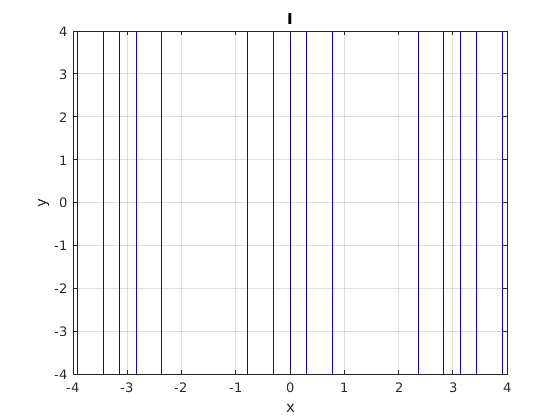
\includegraphics[width=8cm]{14_var_mult_fonct/question1a} \ 
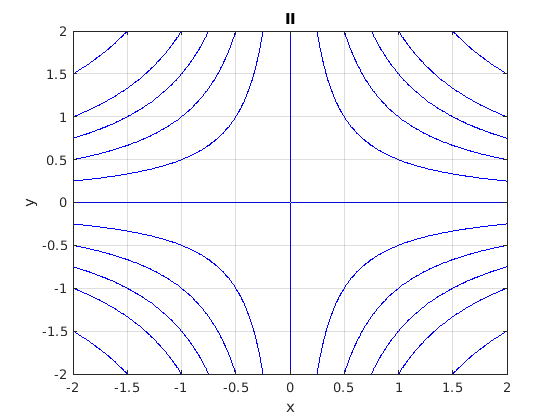
\includegraphics[width=8cm]{14_var_mult_fonct/question1b}

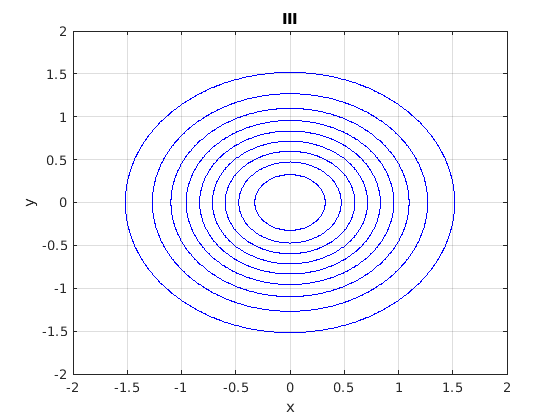
\includegraphics[width=8cm]{14_var_mult_fonct/question1c} \ 
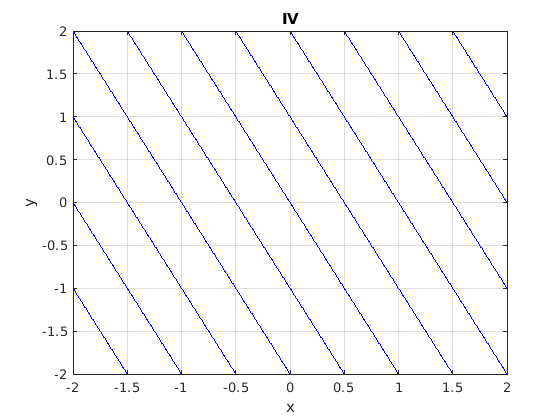
\includegraphics[width=8cm]{14_var_mult_fonct/question1d}

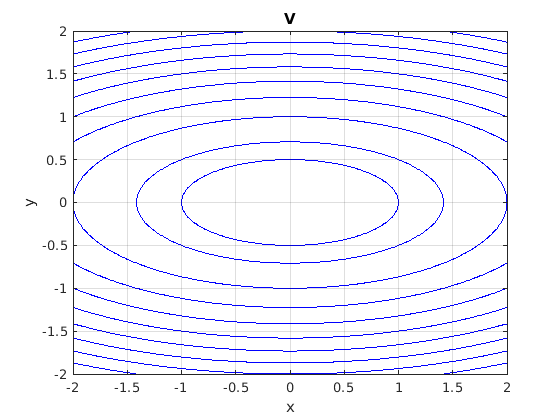
\includegraphics[width=8cm]{14_var_mult_fonct/question1e}
\label{14Q3}
\end{question}

\begin{question}
Trouvez l'équation de plan qui a le diagramme de courbes de niveau
donné ci-dessous.
\MATHgraph{14_var_mult_fonct/question2}{8cm}
\label{14Q4}
\end{question}

\begin{question}
Trouvez l'équation de plan qui produit les données du tableau
suivant.
\begin{center}
\begin{tabular}{|c|c|c|c|}
\hline
$x \diagdown y$ & 10 & 20 & 30 \\
\hline
5 & -22 & -62 & -102 \\
\hline
10 & -7 & -47 & -87 \\
\hline
15 & 8 & -32 & -72 \\
\hline
\end{tabular}
\end{center}
\label{14Q5}
\end{question}

\begin{question}
Trouvez le domaine et l'image, et tracez quelques courbes de niveau
pour chacune des fonctions suivantes.
\begin{center}
\begin{tabular}{*{1}{l@{\hspace{0.5em}}l@{\hspace{6em}}}l@{\hspace{0.5em}}l}
\subQ{a} & $\displaystyle f(x,y) = \ln(1-x^2-2y^2)$ &
\subQ{b} & $\displaystyle f(x,y) = \sqrt{x^2-y^2}$
\end{tabular}
\end{center}
\label{14Q6}
\end{question}

\begin{question}
Dessinez quelques courbes de niveau de la fonction 
\[
f(x,y) = \frac{1}{1+x^2+y^2}
\]
et utilisez ces courbes pour tracer le graphe de la fonction.
\label{14Q7}
\end{question}

\subsection{Fonctions  continues}

\begin{question}
Est-ce que la fonction suivante est continue au point $(0,0)$?
\[
f(x,y) = \begin{cases}
\displaystyle \frac{x\sqrt{y}}{x^2+y} & \text{si}\quad (x,y)\neq (0,0) \\
0 & \text{si}\quad (x,y) = (0,0)
\end{cases}
\]
Justifiez votre réponse.
\label{14Q8}
\end{question}




%%% Local Variables: 
%%% mode: latex
%%% TeX-master: "notes"
%%% End: 
